% Chapter Template

\chapter{Observations} % Main chapter title

\label{Chapter3} % Change X to a consecutive number; for referencing this chapter elsewhere, use \ref{ChapterX}

\lhead{Chapter 3. \emph{Observations}} % Change X to a consecutive number; this is for the header on each page - perhaps a shortened title

%----------------------------------------------------------------------------------------
%    SECTION 1
%----------------------------------------------------------------------------------------
\section{ Introduction}

In this chapter we giving the general over view about the observations used in the study as well as the instrument used to observe them.\\

We used observation from three International LOFAR stations, FR606, SE607 and DE60x. 

\section{LOw Frequency ARray (LOFAR)}
This section based on the full arterial about LOFAR (\citet{van2013lofar})\\

The Low Frequency Array, LOFAR is a unique radio telescope contains number of interferometric array of dipole antenna stations spread in Europe. LOFAR designed and developed by ASTRON, The Netherlands Institute for Radio Astronomy to operate in the low frequency regime of the radio wavelengths, between the 10 to 240 MHz which correspond to the wavelength from 30 to 1.2 m. Beside this, LOFAR also has large field of view, FoV which makes LOFAR an excellent instrument for many key sciences including pulsars and transients. For full details about LOFAR in pulsars and other key science (\citet{ stappers2011observing}). 

LOFAR's stations are mainly distributed in the Netherlands 40 stations and 9 international stations distributed within the partner Europeans countries, 6 in Germany, 3 in Poland and 1 each in France, England, Sweden, Ireland and Italy which joint the International Lofar Telescope, ITL early this year ( see \url{http://www.astron.nl/lofar-crosses-alps-italy-joins}) and Figure (\ref{fig:example1}). These stations are similar to the dishes in the typical radio telescope which can providing raw sensitivity, tracking the sources and collecting area. They classified as the following:

\subsection*{Core Stations}
A set of 24 stations located in the Netherlands with the radius of 
2km. The central region of this core, which contain 6 stations within the area of 320 m diameter is known as Superterp and it gives the shortest baselines for the whole array. All these stations has 96 Low Band Antenna (LBAs) and 48 High Band Antennas (HBAs).Figure (\ref{fig:example1}) showing the Superterp in the central circle of the Core, appear also number of the core stations around it.
\subsection*{Remote Stations}
These are 16 stations distributed approximately as a logarithmic spiral shape over the radius of 90 km. Both, Core and Remote stations distributed over radius of 180 km next to Exloo town in the northeastern Dutch province of Drenthe in the Netherlands.\\
Similar to the Core stations, the Remote stations also have 96 LBAs and 48 HBAs.

\subsection*{International Stations}
Currently, there are 8 functional international LOFAR stations distributed in Germany 5 station and one station of each of France, Sweden (Figure \ref{fig:example}) and England. Each station of these has 96 LBAs and 96 HBAs and 96 digital receiver units (RCUs) which gives total of 192 digital signal path during any single observation.





\begin{figure}[H]
    \centering
    \subfloat[label 1]{{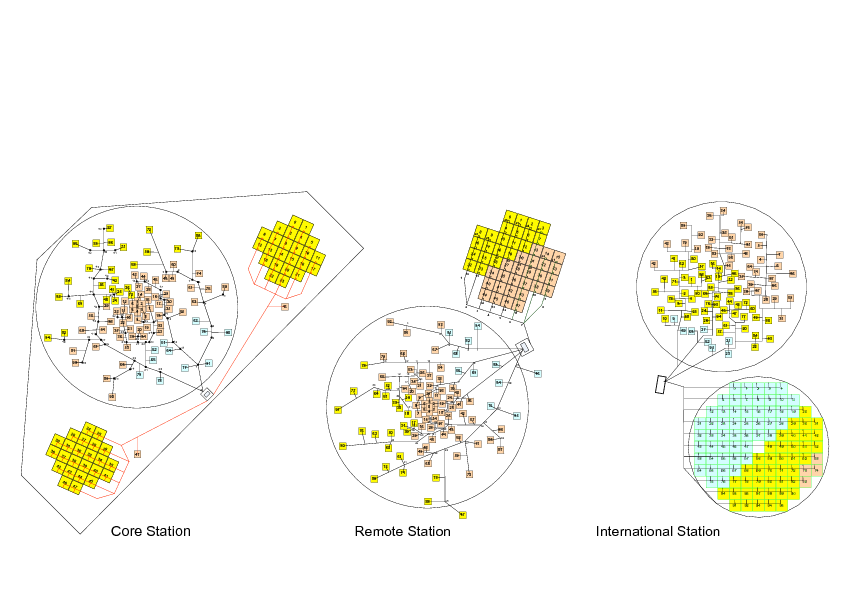
\includegraphics[width=11cm]{figures_LOFAR_stations_02.png} }}%
    \qquad
    \subfloat[label 2]{{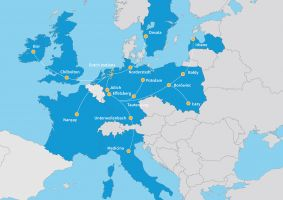
\includegraphics[width=10cm]{LOFAR_Map_2018_0_ITALY.jpg} }}%
    \caption{ (\citet{van2013lofar}) and \url{http://www.astron.nl/lofar-crosses-alps-italy-joins}}%
    \label{fig:example1}%
\end{figure}


\subsection*{High Band Antennas (HBAs)}

\subsection*{Low Band Antennas (LBAs)}



\begin{figure}[H]
    \centering
    \subfloat[Core Stations]{{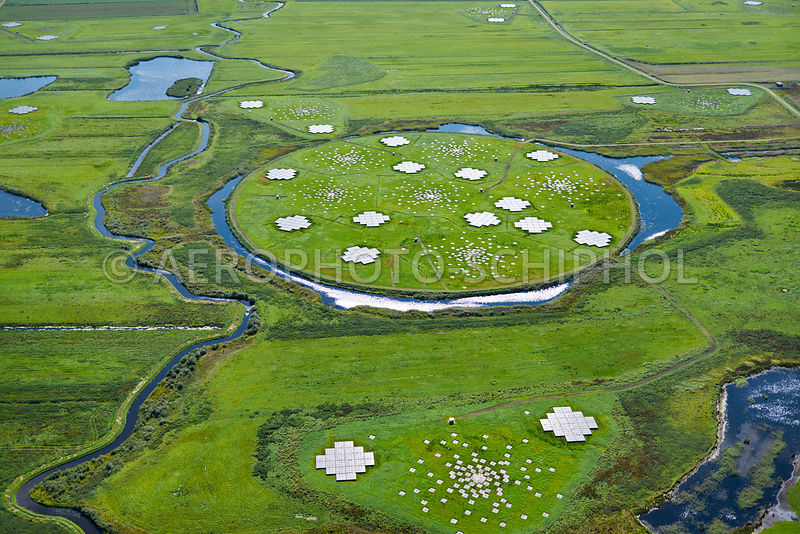
\includegraphics[width=10cm]{301620_xlarge.jpg} }}%
    \qquad
    \subfloat[Sewdish Station]{{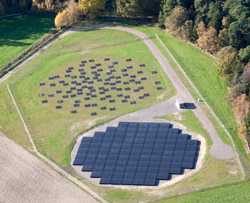
\includegraphics[width=10cm]{ONSALA.jpg} }}%
    \caption{ \citet{gunst2010lofar} and ONSALA (\url{https://www.aerophotostock.com/-/galleries/all/page/59} \url{http://lofar-se.org/})}%
    \label{fig:example}%
\end{figure}











\section{Observations}


\begin{tabular}{SSSSS}\toprule
    {Pulsar} & {B name} & {J name} & {DM ($cm^{-3}pc$)} & {LOFAR Station} \\ \midrule
    1  & {B0320+39}  & {J0141+6009} && FR606 \\
    2  & {B0320+39}  & {J0323+3944} && FR606 \\
    3  & {B1508+55}  & {J1509+5531} && FR606 \\
    4  & {B1737+13}  & {J1740+1311} && FR606 \\
    5  & {B1822-09}  & {J1825-0935} && FR606 \\
    6  & {B1931+24}  & {J1933+2421} && FR606 \\
    7  & {B2016+28}  & {J2018+2839} && FR606 \\
    8  & {B2111+46}  & {J2113+4644} && FR606 \\
    9  & {B2224+65}  & {J2225+6535} && FR606 \\
    10 & {B2310+42}  & {J2313+4253} && FR606 \\
    11 & {B0450+55}  & {J0454+5543} && FR606 \\
    12 & {B0540+23}  & {J0543+2329} && FR606 \\
    13 & {B0809+74}  & {J0814+7429} && FR606 \\
    14 & {B0834+06}  & {J0837+0610} && FR606 \\
    15 & {B0950+08}  & {J0953+0755} && FR606 \\
    16 & {B1133+16}  & {J1136+1551} && FR606 \\
    17 & {B1237+25}  & {J1239+2453} && FR606 \\
    18 & {B1540-06}  & {J1543-0620} && FR606 \\
    19 & {B1642-03}  & {J1645-0317} && FR606 \\
    20 &     {-}     & {J0613+3731} && FR606 \\
    21 & {B0329+54}  & {J0332+5434} && FR606 \\ \bottomrule
\end{tabular}













